% Adapted from PetarV-/TikZ repository @ GitHub
\usetikzlibrary{positioning}

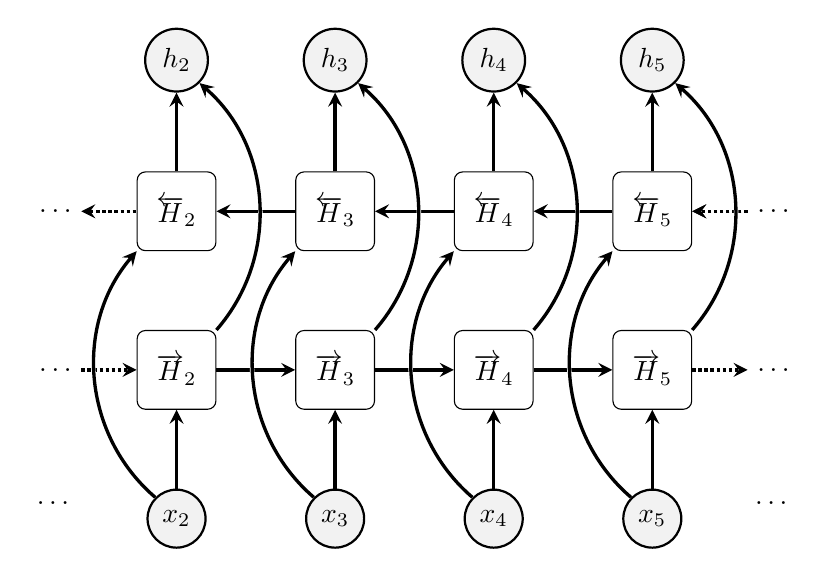
\begin{tikzpicture}[
        inout/.style={circle, draw, fill=gray!10, thick, align=center},
        hid/.style={inner sep=0.2em,rounded corners=0.3em},
    ]
	\node[rectangle] (Y0) at (0, 0) {$\dots$};
    \node[hid, rectangle, draw, right=2em of Y0, minimum height=1cm, minimum width=1cm] (RNN) {$\overrightarrow{H}_{2}$};
    \node[hid, rectangle, right=of RNN, draw, minimum height=1cm, minimum width=1cm] (RNN2) {$\overrightarrow{H}_{3}$};
    \node[hid, rectangle, right=of RNN2, draw, minimum height=1cm, minimum width=1cm] (RNN3) {$\overrightarrow{H}_{4}$};

    \node[hid, rectangle, right= of RNN3, draw, minimum height=1cm, minimum width=1cm] (RNN4) {$\overrightarrow{H}_{5}$};
	\node[rectangle, right=2em of RNN4] (RNN5) {$\dots$};


    \node[hid, rectangle, above=of RNN4, draw, minimum height=1cm, minimum width=1cm] (R25) {$\overleftarrow{H}_{5}$};
    \node[hid, rectangle, left=of R25, minimum height=1cm, minimum width=1cm, draw] (R24) {$\overleftarrow{H}_{4}$};
    \node[hid, rectangle, left=of R24, draw, minimum height=1cm, minimum width=1cm] (R23) {$\overleftarrow{H}_{3}$};
    \node[hid, rectangle, left=of R23, draw, minimum height=1cm, minimum width=1cm] (R22) {$\overleftarrow{H}_{2}$};
    \node[rectangle, left=2em of R22] (R21) {$\dots$};
	\node[right=2em of R25] (Y20) {$\dots$};

	\node[inout, below=of RNN] (X1) {$x_2$};
	\node[inout, below=of RNN2] (X2) {$x_3$};
	\node[inout, below=of RNN3] (X3) {$x_4$};
	\node[inout, below=of RNN4] (X4) {$x_5$};
	\node[inout, above=of R25] (Y5) {$h_5$};
	\node[inout, above=of R24] (Y4) {$h_4$};
	\node[inout, above=of R23] (Y3) {$h_3$};
	\node[inout, above=of R22] (Y2) {$h_2$};

	\draw[-stealth, very thick] (X1) -- (RNN);
	\draw[-stealth, very thick] (X2) -- (RNN2);
	\draw[-stealth, very thick] (X3) -- (RNN3);
	\draw[-stealth, very thick] (X4) -- (RNN4);
	\draw[-stealth, very thick, densely dotted] (Y0) -- (RNN);
	\draw[-stealth, very thick] (RNN) -- (RNN2);
	\draw[-stealth, very thick] (RNN2) -- (RNN3);
	\draw[-stealth, very thick] (RNN3) -- (RNN4);
	\draw[-stealth, densely dotted, very thick] (RNN4) -- (RNN5);
	\node[below=4em of Y0] (d) {\dots};
	\node[below=4em of RNN5] (d) {\dots};

	\path[-stealth, ultra thick, white] (X1) edge[bend left=45] (R22);
	\path[-stealth, very thick] (X1) edge[bend left=45] (R22);
	\path[-stealth, ultra thick, white] (X2) edge[bend left=45] (R23);
	\path[-stealth, very thick] (X2) edge[bend left=45] (R23);
	\path[-stealth, ultra thick, white] (X3) edge[bend left=45] (R24);
	\path[-stealth, very thick] (X3) edge[bend left=45] (R24);
	\path[-stealth, ultra thick, white] (X4) edge[bend left=45] (R25);
	\path[-stealth, very thick] (X4) edge[bend left=45] (R25);
	\draw[-stealth, densely dotted, very thick] (Y20) -- (R25);

	\draw[-stealth, very thick] (R22) -- (Y2);
	\draw[-stealth, very thick] (R23) -- (Y3);
	\draw[-stealth, very thick] (R24) -- (Y4);
	\draw[-stealth, very thick] (R25) -- (Y5);

	\draw[stealth-, densely dotted, very thick] (R21) -- (R22);
	\draw[stealth-, very thick] (R22) -- (R23);
	\draw[stealth-, very thick] (R23) -- (R24);
	\draw[stealth-, very thick] (R24) -- (R25);
	\draw[-stealth, densely dotted, very thick] (Y20) -- (R25);

	\path[-stealth, ultra thick, white] (RNN) edge[bend right=45] (Y2);
	\path[-stealth, very thick] (RNN) edge[bend right=45] (Y2);
	\path[-stealth, ultra thick, white] (RNN2) edge[bend right=45] (Y3);
	\path[-stealth, very thick] (RNN2) edge[bend right=45] (Y3);
	\path[-stealth, ultra thick, white] (RNN3) edge[bend right=45] (Y4);
	\path[-stealth, very thick] (RNN3) edge[bend right=45] (Y4);
	\path[-stealth, ultra thick, white] (RNN4) edge[bend right=45] (Y5);
	\path[-stealth, very thick] (RNN4) edge[bend right=45] (Y5);
\end{tikzpicture}
